\documentclass{article}

\usepackage{graphicx}
\usepackage[french]{babel}
\usepackage[T1]{fontenc}
\usepackage[lined, boxed, commentsnumbered, ruled, vlined, linesnumbered, french, onelanguage]{algorithm2e}
\usepackage{amsfonts}
\usepackage{amsthm}
\usepackage{amsmath}
\usepackage{amssymb}
\usepackage{hyperref}
\usepackage{listings}
\lstset{language=C}
\usepackage{minted}
\usepackage{dirtree}
\usepackage{multirow}
\usepackage{tabularx}
\usepackage{geometry}
\usepackage{pdflscape}

\newtheorem{proposition}{Proposition}
\newtheorem{lemma}{Lemme}
\theoremstyle{definition}
\newtheorem{definition}{Définition}
\newtheorem{notation}{Notation}
\theoremstyle{remark}
\newtheorem{remark}{Remarque}
\newtheorem{example}{Exemple}

\title{Décodage de codes de Reed-Solomon par l'algorithme de Gao}
\author{ABED Walid \and MARCOU Corentin}

\begin{document}

\maketitle

\tableofcontents

\section{Introduction}
\label{sec:intro}

Les codes correcteurs d'erreurs sont des techniques de codage de l'information qui visent à corriger les erreurs qui peuvent arriver durant la transmission. Pour cela, ils se basent sur l'ajout de redondance. Un code notable est celui mis au point par Irving S. Reed et Gustave Solomon en 1960 \cite{RS1960}. Le code de Reed-Solomon est très populaire, on le retrouve dans les CDs, les DVDs, les QR-codes, les communications satellites, etc. En effet, ils sont intéressants en raison de leur grande capacité de correction et leur efficacité en pratique. 

Dans ce rapport, on présente une méthode pour décoder les codes de Reed-Solomon due à Suhong Gao en 2003 \cite{Gao2003}. Pour cela, dans une première partie, on présente quelques généralités sur les codes linéaires. Dans une seconde partie, on définit le code de Reed-Solomon et on explique comment encoder et décoder. Ensuite, dans un troisième temps, on propose une implémentation en C. Finalement, dans une dernière partie, on discute des performances de l'implémentation proposée.

\section{Codes linéaires}
\label{sec:lin}

Dans cette partie, on définit les codes linéaires ainsi que leurs propriétés. On présente un exemple simple pour illustrer: le code de Hamming.

\subsection{Quelques définitions}
\label{subsec:lin-def}

\begin{definition}
\label{def1}
    Soient $A^n$ l'ensemble des mots de longueur $n$ sur l'alphabet $A$, $x = (x_{0}, x_{1}, \dots, x_{n-1}), y = (y_{0}, y_{1}, \dots, y_{n-1}) \in A^n$, la distance de Hamming entre $x$ et $y$ est
    \[d_H(x, y) = \#\{i | i \in \{0, 1, \dots, n-1\}, x_i \ne y_i\} \]
    De plus, si $A$ est un groupe, le poids de Hamming de $x$ est
    \[ w_H(x) = d_H(0, x) \]
\end{definition}

\begin{definition}
\label{def2}
    Un code $C$ sur un alphabet $A$ est une partie non vide de $A^n$. On dira que $n$ est la longueur du code $C$ et que les éléments de $C$ sont les mots de code.  
\end{definition}

\begin{definition}
\label{def3}
    Soit un code $C$ sur $A$,
    \[ d = min\{d_H(x, y) | x, y \in C, x\ne y \}\]
    est la distance minimal du code $C$.
\end{definition}

\begin{remark}
    Il est utile de représenter un code par ses paramètres:
    \begin{itemize}
        \item son alphabet de cardinal $q$
        \item sa longueur $n$
        \item son cardinal $M$
        \item sa distance minimal $d$
    \end{itemize}
    On note alors $C[q, n, M, d]$ un code avec de tels paramètres.
\end{remark}

\begin{definition}
\label{def4}
    Soit un code $C$ sur $A$, on dit que $C$ est linéaire sur $A$ si $A$ est un corps et $C$ un sous-espace vectoriel de $A^n$. De plus la dimension de $C$ comme sous-espace vectoriel de $A^n$ est alors appelée la dimension du code $C$. On notera alors $C[q, n, k, d]$ plutôt que $C[q, n, q^k, d]$.
\end{definition}

\begin{definition}
    Soient $x \in A^n$, $r \in \mathbb{N}$ on appelle boule de Hamming l'ensemble
    \[ \mathcal{B}_H(x, r) = \{y \in A^n | d_H(x, y) \le r\} \]
\end{definition}

\begin{proposition}
    Pour un code de distance minimale $d$, les boules de Hamming $\{ \mathcal{B}_H(c, \lfloor \frac{d-1}{2} \rfloor) | c \in C\}$ sont disjointes.
\end{proposition}

\begin{proof}
    Soient $c, c' \in C$ distincts. Par l'absurde, on suppose qu'il existe $x \in C$ tel que $x \in \mathcal{B}_H(c, \lfloor \frac{d-1}{2} \rfloor)$ et $x \in \mathcal{B}_H(c', \lfloor \frac{d-1}{2} \rfloor)$. Ainsi,
    \begin{align*}
        d_H(c, c') &\le d_H(c, x) + d_H(c', x) \\
                   &\le \lfloor \frac{d-1}{2} \rfloor + \lfloor \frac{d-1}{2} \rfloor \\
                   &\le \frac{d-1}{2} + \frac{d-1}{2} \\
                   &\le d - 1 \\
                   &< d 
    \end{align*}
    Or, $c$ et $c'$ sont des mots de code donc $d_H(c, c') \ge d$. Contradiction.
\end{proof}

\begin{remark}
    Un code de distance minimale $d$ peut corriger au plus $\lfloor \frac{d-1}{2} \rfloor$ erreurs.
\end{remark}

\begin{remark}
    On peut définir une procédure simple de décodage: le décodage par vraisemblance maximale. Pour cela à tout $x \in A^n$, on associe le mot de code $c \in C$ qui maximise la probabilité $\mathbb{P}(x | c)$. 
\end{remark}

\begin{proposition}[Borne de Singleton]
\label{prop1}
    Soit un code linéaire $C[q, n, k, d]$ alors
    \[ k + d \le n + 1 \]
\end{proposition}

\begin{proof}
    On considère l'application
    \[ 
    \begin{array}{cccc}
         \phi: & \mathbb{F}_q^n & \longrightarrow & \mathbb{F}_q^{n-(d-1)}\\
         & (x_1, \dots, x_n) & \longmapsto & (x_1, \dots, x_{n-(d-1)})
    \end{array}
    \]
    On remarque que $dim(Im(\phi)) = n - (d-1)$. On doit montrer que $\phi \vert_{C}$ est injective, pour cela, on montre que $ker(\phi \vert_{C}) = {0}$. Soit $c \in C$ tel que $\phi(c) = 0$, i.e, $c_1 = c_2 = \dots = c_{n-(d-1)} = 0$. On a alors $w_H(c) \le d - 1$ donc $c = 0$. Et
    \[
        \underbrace{dim(ker(\phi \vert_{C}))}_{= 0} + \underbrace{dim(Im(\phi \vert_{C})}_{\le n-(d-1)} = k 
    \]
\end{proof}

\begin{definition}
\label{def5}
    On appelle matrice génératrice du code $C$ toute matrice $\mathcal{G} \in \mathcal{M}_{l \times n}$ avec $l \ge k$ telle que 
    \[ C = \{ m \mathcal{G} | m \in \mathbb{F}_q^l \}. \]
\end{definition}

\begin{definition}
\label{def6}
    On appelle matrice de parité ou de contrôle toute matrice $\mathcal{H} \in \mathcal{M}_{n-l \times n}$ avec $l \ge k$ dont le noyau est $C$, autrement dit,
    \[ C = \{ x \in \mathbb{F}_{q^n} | \mathcal{H}x^T = 0 \} \]
\end{definition}

\begin{definition}
    Soit $x \in \mathbb{F}_q^n$, le syndrome de $x$ est
    \[ S(x) = Hx^T \in \mathbb{F}_q^{n-k} \]
    On a donc $S(x) = 0$ si et seulement si $x \in C$. $H$ induit une relation d'équivalence $\mathcal{R}$  sur $\mathbb{F}_q^n$: $x\mathcal{R}y \Leftrightarrow S(x) = S(y)$.  
\end{definition}

\begin{proposition}
    Il existe au plus un mot de poids $\le \lfloor \frac{d-1}{2} \rfloor$ dans une classe d'équivalence.
\end{proposition}

\begin{proof}
    Soient $x, y \in \mathbb{F}_q^n$ tels que $x \mathcal{R} y$, $w_H(x) \le \lfloor \frac{d-1}{2} \rfloor$ et $w_H(y) \le \lfloor \frac{d-1}{2} \rfloor$. Alors $x - y \in C$ et $w_H(x - y) = d_H(x, y) \le d_H(x, 0) + d_H(y, 0) = w_H(x) + w_H(y) \le  \lfloor \frac{d-1}{2} \rfloor + \lfloor \frac{d-1}{2} \rfloor \le \frac{d-1}{2} + \frac{d-1}{2} \le d - 1 < d$. Donc $x - y = 0$, d'où $x = y$. 
\end{proof}

\begin{remark}
    On peut se servir de la matrice de parité et du syndrome pour définir un algorithme de décodage. Pour toute classe d'équivalence, on choisit l'élément de plus petit poids de Hamming comme représentant. Il suffit alors de calculer le syndrome de $x$ puis de trouver le plus petit représentant de sa classe d'équivalence, on le note $y$. On renvoie alors $x - y$. 
\end{remark}

\subsection{Un exemple: le code de Hamming}
\label{subsec:lin-ham}

Soit un entier $l \ge 3$, on considère la matrice $H_l$ à $l$ lignes et $2^l - 1$ colonnes qui est la concaténation de tous les mots de binaires de tailles $l$ non nuls.

\begin{example}
    Pour $l = 3$,
    \[ H_3 = 
    \begin{pmatrix}
        1 & 0 & 0 & 1 & 1 & 0 & 1 \\
        0 & 1 & 0 & 1 & 0 & 1 & 1 \\
        0 & 0 & 1 & 0 & 1 & 1 & 1
    \end{pmatrix}
    \]
\end{example}

\begin{proposition}
\label{prop2}
    Un code de Hamming paramétré par $l \ge 3$ a pour paramètres $[2, 2^l - 1, 2^l -l - 1,3]$ et pour matrice de parité $H_l$. On note un tel code $C_l$.
\end{proposition}

\begin{proof}
    On considère l'application associée à $H_l$
    \[ 
    \begin{array}{cccc}
         \phi: & \mathbb{F}_2^{2^l - 1} & \longrightarrow & \mathbb{F}_2^l\\
         & x & \longmapsto & H_lx^T
    \end{array}
    \]
    Comme $H_l$ est la matrice de parité du code, on a $ker(\phi) = C_l$. De plus
    \[dim(ker(\phi)) + dim(Im(\phi)) = 2^l - 1.\]
    Donc
    \[dim(C_l) + rg(H_l) = 2^l - 1.\]
    Il suffit alors de montrer que $rg(H_l) = l$, pour cela, on sélectionne $l$ colonnes de $H_l$ qui forment une matrice de permutation.

    Pour ce qui est de la distance minimale, il suffit de voir que $H_l$ n'a pas de colonne nulle donc $d > 1$, n'a pas de colonnes identiques donc $d > 2$ et qu'il est aisé de trouver trois colonnes donc la somme est nulle, d'où $d = 3$.
\end{proof}

\begin{remark}
    Voici un algorithme de décodage pour ce code.
    \begin{algorithm}
    \caption{Algorithme de décodage du code de Hamming}
        \Entree{$x = (x_0, \dots, x_{2^l-1}) \in \mathbb{F}_2^{2^l -1}$}
        \Sortie{$c \in C$ mot de code correspondant}
        $s \gets H_lx^T$ \\
        \eSi{$s = 0$}
        {
            $x \in C$ \\
            \Retour{$x$}
        }
        {
            $s$ est la $i$-ème colonne de $H_l$ \\
            \Retour{$c = (x_0, \dots, x_{i-1}, 1 + x_i, x_{i+1}, \dots, x_{2^l - 1})$}
        }
        
    \end{algorithm}
\end{remark}

\section{Codes de Reed-Solomon}
\label{sec:rs}

On s'intéresse désormais au code de Reed-Solomon. Dans cette partie, on donne une définition et on présente un algorithme de décodage.

\subsection{Présentation}
\label{sec:rs-pre}

Soient $q$ une puissance d'un nombre premier, $n$ et $k$ deux entiers tels que $ 1 \le k < n \le q$, $a = (a_{1}, a_{2}, \dots, a_{n}) \in \mathbb{F}_{q}^{n}$ avec les $a_{i}$ distincts, on note
\[ RS_{k}(a) = \{ (f(a_{1}), f(a_{2}), \dots, f(a_{n}) | f \in \mathbb{F}_{q}[X], deg(f) < k \} \]

Dans la suite, on notera $\mathbb{F}_{q}[X]_{< k}$ les polynômes à coefficients dans $F_q$ de degré strictement inférieur à $k$.

\begin{proposition}
\label{prop3}
    $RS_{k}(a)$ a pour paramètres $[q, n, k, d]$, avec $d = n-k+1$
\end{proposition}

\begin{proof}
    On veut montrer que la dimension du code est $k$, pour cela, on considère
    \[ 
    \begin{array}{cccc}
        \phi_{k,a}: & \mathbb{F}_{q}[X]_{< k} & \longrightarrow & \mathbb{F}_{q}^{n}\\
        & f & \longmapsto & (f(a_{1}), \dots, f(a_{n}))
    \end{array}
    \]
    On note que $\mathbb{F}_{q}[X]_{< k}$ est un $\mathbb{F}_{q}$ espace vectoriel de dimension $k$. De plus, on remarque que
    \[ Im(\phi_{k,a}) = RS_{k}(a). \] 
    On peut alors écrire,    
    \[ dim(RS_{k}(a)) = dim(Im(\phi_{k,a})) = k. \]
    On a
    \[ dim(Im(\phi_{k,a})) + dim(ker(\phi_{k,a})) = k. \]
    Il suffit donc de montrer que $\phi_{k,a}$ est injective. Soit $f \in \mathbb{F}_{q}[X]_{< k}$ tel que $f(a_{1}) = f(a_{2}) = \dots = f(a_{n}) = 0$. Donc $f$ a $n$ racines distinctes et $deg(f) < k < n$. D'où $f = 0$.

    On veut montrer que la distance minimale du code est $n-k+1$. Soit $c = (f(a_{1}), \dots, f(a_{n})) \in RS_{k}(a)$ un mot de code non nul. $f \ne 0$ a au plus $k-1$ racines distinctes. Ainsi le mot de code est non nul sur au moins $n - (k - 1)$ points. 
\end{proof}

\begin{remark}
    Les codes de Reed-Solomon atteignent la borne de Singleton \ref{prop1}, on dit qu'ils sont MDS (Maximum Distance Separable).
\end{remark}

\begin{remark}
    Une matrice génératrice de $RS_{k}(a)$ est
    \[ \begin{pmatrix}
        1 & 1 & \cdots & 1 \\
        a_{1} & a_{2} & \cdots & a_{n} \\
        a_{1}^2 & a_{2}^2 & \cdots & a_{n}^2 \\
        \vdots & \vdots & \ddots & \vdots \\
        a_{1}^{k-1} & a_{2}^{k-1} & \cdots & a_{n}^{k-1} \\
    \end{pmatrix} \]
\end{remark}

\subsection{Encodage}
\label{subsec:rs-enc}

Pour calculer le mot de de code d'un message, il suffit de définir le polynôme associé au message et de l'évaluer en chaque point. Formellement,

\begin{algorithm}
\label{algo1}
\caption{Algorithme d'encodage du code de Reed-Solomon}

\Entree{$a = (a_{1}, a_2, \dots, a_n) \in \mathbb{F}_{q}$, un message $m = (m_{1}, m_{2}, \dots, m_{k}) \in \mathbb{F}_{q}^{k}$}
\Sortie{un mot de code $c = (c_{1}, c_{2}, \dots, c_{n}) \in \mathbb{F}_{q}^{n}$}

$f \gets m_{1} + m_2x + \cdots + m_kx^{k-1}$ \\
\Pour{$i$ allant de $1$ à $n$}{
    $c_i \gets f(a_i)$\;
}
\Retour $(c_{1}, c_2, \dots, c_n)$
\end{algorithm}

\subsection{Décodage}
\label{subsec:rs-dec}

On remarque que pour décoder un mot de code (donc un message reçu sans erreurs), il suffit de réaliser une interpolation pour retrouver le polynôme $f$.
On décrit désormais une procédure de décodage présentée par Shuhong Gao en 2002. On reçoit un message $b = (b_{1}, b_2, \dots, b_n)$ associé à un mot de code $c = (c_{1}, c_2, \dots, c_n)$ avec $t$ erreurs, $t \leq \frac{d-1}{2}$. On souhaite inverser la procédure de codage, c'est-à-dire, retrouver le polynôme $f$ associé au message $m$ comme dans l'algorithme \ref{algo1}. Pour cela, on pré-calcule le polynôme
\[ g_{0} = \prod_{i = 1}^{n} (x - a_i). \]
On peut alors appliquer la procédure suivante

\begin{algorithm}[H]
\label{algo2}
\caption{Algorithme de décodage du code de Reed-Solomon \cite{Gao2003}}
\Entree{un message reçu $b = (b_{1}, b_2, \dots, b_n) \in \mathbb{F}_q^n$}
\Sortie{un polynôme $m_{1} + m_2X + \cdots + m_kX^{k-1} \in \mathbb{F}_q[X]$ ou "Erreur"}
$g_{1} \gets$ Interpolation($b_{1}, b_2, \dots, b_n$) \\
$u, v, g \gets$ PGCDpartiel($g_{0}, g_{1}, \frac{n+k}{2}$) \\
$f, r \gets$ DivisionEuclidienne($g$, $v$) \\
\eSi{$r = 0$ et $deg(f) < k$}{
    \Retour{$f$}
}{
    \Retour{"Erreur"}
}
\end{algorithm}

\vspace{0.5cm}

Pour expliquer pourquoi la méthode fonctionne, on suit la même démarche que Gao \cite{Gao2003}, on commence par un rappel sur l'algorithme d'Euclide étendu. Soient $r_{0}, r_{1} \in \mathbb{F}_q[X]$ non nuls, on pose
\[ u_{0} = 1 \text{, } u_{1} = 0 \text{, } v_{0} = 0 \text{, } v_{1} = 1 \]
Durant l'exécution de l'algorithme, on peut observer les relations de récurrence suivantes
\begin{equation}
\label{eq:euc1}
    r_{i-1} = q_{i}r_{i} + r_{i+1}
\end{equation}
où $deg(r_{i+1} < deg(r_i)$ pour $i = 1, 2 \dots, n$, $r_i \ne 0$ pour $i = 0, 1, \dots, n$ et $r_{m+1} = 0$ et
\begin{equation}
\label{eq:euc2}
    u_{i+1} = u_{i-1} - q_{i}u_{i} \text{, } v_{i+1} = v_{i-1} - q_{i}v_{i}
\end{equation}
pour $i = 1, 2 \dots, m$.
L'algorithme d'Euclide nous donne le résultat $pgcd(r_{0}, r_{1}) = r_m$. On a aussi
\begin{equation}
\label{eq:euc3}
    r_i = u_{i}r_{0} + v_{i}r_{1} \text{, } i = 1, 2 \dots, m.
\end{equation}
Les deux lemmes suivants seront utiles pour montrer la correction de l'algorithme \ref{algo2}.

\begin{lemma}
\label{lem1}
    Avec les notations ci-dessus, on a
    \[ u_{m+1} = (-1)^{m+1} \frac{r_{1}}{r_{m}} \text{ et } v_{m+1} = (-1)^{m} \frac{r_{0}}{r_{m}} \]
\end{lemma}

\begin{proof}
    En réécrivant les relation \ref{eq:euc2} sous forme matricielle, on a
    \[
    \begin{pmatrix}
        u_{i} & v_{i} \\
        u_{i+1} & v_{i+1}
    \end{pmatrix}
    =
    \begin{pmatrix}
        0 & 1 \\
        1 & -q_{i}
    \end{pmatrix}
    \begin{pmatrix}
        u_{i-1} & v_{i-1} \\
        u_{i} & v_{i}
    \end{pmatrix}.
    \]
    On remarque alors
    \[
    \begin{pmatrix}
        u_{i} & v_{i} \\
        u_{i+1} & v_{i+1}
    \end{pmatrix}
    = 
    \begin{pmatrix}
        0 & 1 \\
        1 & -q_{i}
    \end{pmatrix}
    \begin{pmatrix}
        0 & 1 \\
        1 & -q_{i-1}
    \end{pmatrix}
    \dots
    \begin{pmatrix}
        0 & 1 \\
        1 & -q_{1}
    \end{pmatrix}
    \begin{pmatrix}
        u_0 & v_0 \\
        u_1 & v_1
    \end{pmatrix}.
    \]
    Or comme,
    \[
    \begin{pmatrix}
        u_0 & v_0 \\
        u_1 & v_1
    \end{pmatrix}
    = 
    \begin{pmatrix}
        1 & 0 \\
        0 & 1
    \end{pmatrix}
    \]
    on a
    \[
    \begin{vmatrix}
        u_{i} & v_{i} \\
        u_{i+1} & v_{i+1}
    \end{vmatrix}
    = u_{i}v_{i+1} - v_{i}u_{i+1} = 
    \prod_{j=1}^i
    \begin{vmatrix}
         0 & 1 \\
        1 & -q_{j}
    \end{vmatrix}
    = (-1)^i
    \]
    Par ailleurs, on peut aussi traduire la relation \ref{eq:euc3} matriciellement,
    \[
    \begin{pmatrix}
        r_i \\
        r_{i+1}
    \end{pmatrix}
    =
    \begin{pmatrix}
        u_{i} & v_{i} \\
        u_{i+1} & v_{i+1}
    \end{pmatrix}
    \begin{pmatrix}
        r_0 \\
        r_1
    \end{pmatrix}.
    \]
    Ainsi, 
    \[\begin{pmatrix}
        r_0 \\
        r_1
    \end{pmatrix}
    =
    \begin{pmatrix}
        u_{i} & v_{i} \\
        u_{i+1} & v_{i+1}
    \end{pmatrix} ^ {-1}
    \begin{pmatrix}
        r_i \\
        r_{i+1}
    \end{pmatrix}
    =
    (-1)^i
    \begin{pmatrix}
        v_{i+1} & -v_{i} \\
        -u_{i+1} & u_{i}
    \end{pmatrix}
    \begin{pmatrix}
        r_i \\
        r_{i+1}
    \end{pmatrix}.
    \]
    En prenant $i = m$, on obtient donc
    \[ u_{m+1} = (-1)^{m+1} \frac{r_{1}}{r_{m}} + u_{m}r_{m+1} \text{ et } v_{m+1} = (-1)^{m} \frac{r_{0}}{r_{m}} + v_{m}r_{m+1} \]
    On conclut en remarquant que $r_{m+1} = 0$.
\end{proof}

\begin{lemma}
\label{lem2}
    Soient $g_0, g_1 \in \mathbb{F}_q[X]$ tels que
    \[ g_0 = w r_0 + \epsilon_0 \text{ et } g_1 = w r_1 + \epsilon_1 \]
    où $w, r_i, \epsilon_i \in \mathbb{F}_q[X]$, $deg(r_i) \le t$, $deg(\epsilon_i) \le l$ pour $i = 0, 1$ et $pgcd(r_0, r_1) = 1$.
    On suppose qu'il existe un entier $d$ tel que
    \[ l + t < d \le deg(w). \]
    On applique l'algorithme d'Euclide étendu partiel à $g_0$ et $g_1$, on s'arrête quand le degré du reste $g$ a un degré strictement inférieur à $d$. On a à l'arrêt
    \[ ug_0 + vg_1 = g. \]
    Alors, on a
    \[ u = -\alpha r_1 \text{ et } v = \alpha r_0 \]
    où $\alpha \in \mathbb{F}_q^*$.
\end{lemma}

\begin{proof}
    On commence par montrer que l'algorithme d'Euclide étendu calcule la même suite de quotient pour $(r_0, r_1)$ et pour $(g_0, g_1)$. On rappelle
    \[ r_{i-1} = q_i r_i + r_{i+1} \text{ avec } deg(r_{i+1}) < deg(r_i) \text{, } i = 1, 2, \dots, m \]
    et $r_{m+1} = 0$ et $r_m \in \mathbb{F}_{q}^*$. On définit
    \[ u_0 = 1 \hspace{1cm}  u_1 = 0 \hspace{1cm} u_{i+1} = u_{i-1} - q_i u_i \]
    \[ v_0 = 0 \hspace{1cm} v_1 = 1 \hspace{1cm} v_{i+1} = v_{i-1} - q_i v_i \]
    alors
    \[ r_i = u_i r_0 + v_i r_1. \]
    Par le lemme \ref{lem1}, on a
    \[ u_{m+1} = (-1)^{m+1} \frac{r_1}{r_m} \text{ et } v_{m+1} = (-1)^{m} \frac{r_0}{r_m} \]
    On pose
    \[ g_i = u_i g_0 + v_i g_1 \]
    On a alors
    \begin{align*}
        q_i g_i + g_{i+1} &= q_i (u_i g_0 + v_i g_1) + u_{i+1} g_0 + v_{i+1} g_1 \\
        &= q_i (u_i g_0 + v_i g_1) + (u_{i-1} - q_i u_i) g_0 + (v_{i-1} - q_i v_i) g_1 \\
        &= u_{i-1} g_0 + v_{i-1} g_1 \\
        &= g_{i-1}.
    \end{align*}
    Il nous reste à montrer que les degrés de $g_1, \dots, g_{m+1}$ sont strictement décroissants. 
    Pour cela, on écrit
    \begin{align*}
        g_i &= u_i(w r_0 + \epsilon_0) + v_i(w r_1 + \epsilon_1) \\
        &= w (u_i r_0 + v_i r_1) + (u_i \epsilon_0 + v_i \epsilon_1) \\
        &= w r_i + (u_i \epsilon_0 + v_i \epsilon_1) 
    \end{align*} 
    Par ailleurs, on remarque que
    \[ deg(u_i) \le deg(r_1) \le t \text{ et } \deg(v_i) \le deg(r_0) \le t. \]
    D'où
    \[ deg(u_i \epsilon_0 + v_i \epsilon_1) \le l + t < d \le deg(w). \]
    Ainsi, on a
    \begin{align*}
        deg(g_i) &= deg(w) + deg(r_i) \ge deg(w) \ge d > l + t \\
        deg(g_{m+1}) &= deg(u_{m+1} \epsilon_0 + v_{m+1} \epsilon_1) \le l + t.
    \end{align*}
    On sait que les degrés de $r_1, \dots, r_m$ sont strictement décroissant donc par les relations ci-dessus, les degrés de $g_1, \dots, g_{m+1}$ le sont aussi. Ainsi, jusqu'à l'étape $m$, les quotients calculés par l'algorithme d'Euclide étendu pour $(g_0, g_1)$ sont $q_1, \dots, q_m$, c'est donc aussi le cas pour les $u$ et $v$. Ainsi l'étape $m$ est la première étape où le reste $g_{m+1}$ a une degré $<d$ et on a
    \[ g_{m+1} = u_{m+1} g_0 + v_{m+1} g_1 \]
    $u_{m+1}$ et $v_{m+1}$ sont bien de la forme recherchée.
\end{proof}

\begin{proposition}
\label{prop4}
    Si le message reçu $b = (b_1, b_2, \dots, b_n)$ a au plus $ \lfloor \frac{d-1}{2} \rfloor$ erreurs alors l'algorithme retourne bien le polynôme $f$ associé au message $m$.
\end{proposition}

\begin{proof}
    On note $t$ la distance de $b$ à l'unique mot de code $c$ (le nombre d'erreurs). On a donc $t \le \frac{d-1}{2}$.
    On définit le polynôme localisateur d'erreur
    \[ w(x) = \prod_{1 \le i \le n, c_i \ne b_i} (x - a_i) \]
    donc $deg(w) = t$. De plus, on pose
    $w_0 = \frac{g_0}{w}$ et $\Bar{w}$ l'unique polynôme de degré strictement inférieur à t tel que
    \[ \Bar{w} = \frac{b_i - c_i}{w_0(a_i)}, \forall 1 \le i \le n \text{ tel que } b_i \ne c_i. \]
    Alors $w$ et $\Bar{w}$ sont premiers entre eux et $ g_1 = w_0 \Bar{w} + f$ car les deux polynômes ont un degrés inférieurs à $n$ et prennent les même valeurs quand on les évalue en $a_i$
    \begin{align*}
        w_0(a_i) \Bar{w}(a_i) + f(a_i) &= w_0(a_i) \frac{b_i - c_i}{w_0(a_i)} + c_i \\
        &= b_i \\
        &= g_1(b_i) \text{ par définition.}
    \end{align*}
    De plus, on pose $d_0 = \frac{n + k}{2}$. On constate que
    \[ deg(w_0(x)) = deg(g_0) - deg(w) = n - t \ge d_0 \ge k - 1 + t \ge deg(f) + deg(w). \]
    Donc en utilisant le lemme \ref{lem2}, on a $u = -\alpha \Bar{w}$ et $v = \alpha w$, $\alpha \in \mathbb{F}_q^*$. Donc
    \begin{align*}
        g &= u g_0 + v g_1 \\
          &= (-\alpha \Bar{w}) (w_0 w) + (\alpha w) (w_0 \Bar{w} + f) \\
          &= vf
    \end{align*}
    Donc à la ligne 4 de l'algorithme \ref{algo2} le reste sera nul et on a bien le polynôme associé au message.

    On suppose désormais que l'algorithme retourne un polynôme $f$. Comme $deg(f) < k$, f est bien associé à un mot de code. De plus, en combinant les lignes $2$ et $3$ de \ref{algo2}, on a
    \[ g = fv \implies ug_0 = v(f - g_1). \]
    Donc, par définition de $g_0$
    \[ v(a_i)(f(a_i) - g_1(a_i)) = 0, \hspace{3mm} i = 1, 2, \dots, n. \]
    Or $deg(v) \le \frac{d-1}{2}$, on a alors que $f(a_i) = g(a_i)$ pour au moins $n-\frac{d-1}{2}$ valeurs. Donc $b$ est à une distance au plus $\frac{d-1}{2}$ du mot de code associé à $f$. Si $b$ est à une distance supérieure à $\frac{d-1}{2}$ de tous les mots de code alors l'algorithme doit retourner une erreur, le décodage étant alors impossible.
    \end{proof}

\section{Implémentation}
\label{sec:impl}

Dans cette partie, on propose une implémentation de l'algorithme de Gao. Pour cela, on commence par donner les algorithmes qu'on a utiliser pour réaliser les différentes étapes. Ensuite, on précise l'architecture de notre programme.

\subsection{Transformée de Fourier}

Pour encoder un message \ref{algo1}, on doit évaluer un polynôme en $n$ points. Avec la méthode d'Horner, l'évaluation d'un polynôme en un point s'effectue en $\mathcal{O}(n)$, et donc en $n$ points en $\mathcal{O}(n^2)$. On peut toutefois faire mieux. En effet, la transformée de Fourier rapide (FFT) évalue un polynôme $f$ au $n$ points $1, \omega, \omega^2, \dots, \omega^{n-1}$ avec une complexité en $\mathcal{O}(n\log{}n)$.  La FFT permet donc de réduire la complexité de l'encodage des codes de Reed-Solomon qui se résume alors à une FFT. Dans cette implémentation, $n$ doit être une puissance de 2 supérieure à $1$ et il doit exister une racine primitive $n$-ième de l'unité. On rappelle l'algorithme de la FFT

\vspace{0.5cm}

\begin{algorithm}[H]
\label{algo_fft}
\caption{Algorithme de la transformée de Fourier rapide \cite{moderncomp}}
\Entree{Un entier $n = 2^k$, un polynôme $F = \sum_{0 \le i < n}f_iX^i $, $\omega, \omega^2, \dots, \omega^{n-1}$ avec $\omega$ une racine primitive $n$-ème de l'unité dans $\mathbb{F}_p$}
\Sortie{$F(1), F(\omega), \dots, F(\omega^{n-1})$}
\Si{$n = 1$}
{
    \Retour{$f_0$}
} 
$k \gets \frac{n}{2}$ \\
$R_0 \gets \sum_{0 \le j < k} (f_j + f_{j+k})X^j$ \\
$R_1^* \gets \sum_{0 \le j < k} (f_j - f_{j+k})\omega^jX^j $ \\
$ R_0(1), R_0(\omega^2), \dots, R_0((\omega^2)^{k-1}) \gets$ FFT($k$, $\omega^2, (\omega^2)^2, \dots, (\omega^2)^{k-1}$, $R_0$)\\
$R_1^*(1), R_1^*(\omega^2), \dots, R_1^*((\omega^2)^{k-1}) \gets$ FFT($k$, $\omega^2, (\omega^2)^2, \dots, (\omega^2)^{k-1}$, $R_1^*$) \\
\Retour{$R_0(1), R_1^*(1), R_0(\omega^2), R_1^*(\omega^2), \dots, R_0((\omega^2)^{k-1}), R_1^*((\omega^2)^{k-1})$}
\end{algorithm}

\vspace{0.5cm}

L'inverse de la FFT permet de faire une interpolation en $\mathcal{O}(n\log{}n)$, alors que la méthode avec les polynômes de Lagrange s'effectue en $\mathcal{O}(n^2)$. Cela permet d'améliorer la complexité de la première étape du décodage \ref{algo2}. Dans cette implémentation, $n$ doit être une puissance de 2 supérieure à $1$ et il doit exister une racine primitive $n$-ième de l'unité.
Cela implique que $2$ est inversible. Dans notre cas, $2^{-1} = \frac{p+1}{2}$.

\vspace{0.5cm}

\begin{algorithm}[H]
\label{algo_inv_fft}
\caption{Algorithme de l'inverse de la transformée de Fourier rapide \cite{moderncomp}}
\Entree{Un entier $n = 2^k$, $\omega, \omega^2, \dots, \omega^{n-1}$ avec $\omega$ une racine primitive $n$-ème de l'unité dans $\mathbb{F}_p$ ainsi que $F(1), F(\omega), \dots, F(\omega^{n-1})$}
\Sortie{$F = \sum_{0 \le i < n}f_iX^i $, l'unique polynôme de degré au plus $n$ respectant les contraintes}
\Si{$n = 1$}
{
    \Retour{$f_0$}
} 
$k \gets \frac{n}{2}$ \\
$R_0(1), R_0(\omega^2), \dots, R_0((\omega^2)^{k-1}) \gets F(1), F(\omega^2), \dots, F(\omega^{n-2})$\\
$R_1^*(1), R_1^*(\omega^2), \dots, R_1^*((\omega^2)^{k-1}) \gets F(\omega), F(\omega^3), \dots, F(\omega^{n-1})$\\
$R_0 \gets $invFFT$(k, \omega^2, (\omega^2)^2, \dots, (\omega^2)^{k-1}, R_0(1), R_0(\omega^2), \dots, R_0((\omega^2)^{k-1})$\\
$R_1^* \gets $invFFT$(k, \omega^2, (\omega^2)^2, \dots, (\omega^2)^{k-1}, R_1^*(1), R_1^*(\omega^2), \dots, R_1^*((\omega^2)^{k-1})$\\
$F \gets \sum_{0 \le j < k} 2^{-1}({R_0}_j + {R_1^*}_j\omega^{n-j})X^j + \sum_{0 \le j < k}  2^{-1}({R_0}_j - {R_1^*}_j\omega^{n-j})X^{j+k}$\\
\Retour{$F$}
\end{algorithm}

\vspace{0.5cm}

\begin{remark}
    La transformée de Fourier permet aussi d'améliorer la complexité de la multiplication de polynômes. En effet, on passe alors d'une complexité quadratique en le degré des polynômes à une complexité quasi-linéaire. Pour cela, il suffit d'appliquer la FFT aux deux polynômes puis de multiplier les évaluations et de reconstruire les coefficients du produit en faisant une interpolation (inverser la FFT). Les polynômes doivent avoir un degré strictement inférieur à $\frac{n}{2}$.
\end{remark}

\subsection{Division euclidienne}

La troisième étape de l'algorithme de Gao \ref{algo2} réalise une division euclidienne. La méthode naïve qui consiste à poser la division d'un polynôme de degré $n$ par un polynôme de degré $m \le n$ s'effectue en $\mathcal{O}(m(n-m+1))$, ou en $\mathcal{O}(n^2)$ dans le pire cas. Il est possible de réduire cette complexité à $\mathcal{O}(n\log{}n\log{}\log{}n)$ avec un algorithme utilisant l'inversion rapide de série formelle.

\subsubsection{Série formelle}

\begin{definition}
    Une série formelle à coefficient dans un anneau $A$ est de la forme $\sum_{i \in \mathbb{N}} a_i X^i$.
    On note $A[[X]]$ l'anneau des séries formelles et on défini
    \[ P + Q = \sum_{i \in \mathbb{N}} (p_i + q_i) X^i \text{ et } PQ = \sum_{i \in \mathbb{N}} (p_i q_i) X^i\]
\end{definition}

On veut donc une méthode qui permet de calculer l'inverse d'une série formelle, i.e, trouver une série formelle $Q$ tel que $PQ = 1$. Le résultat suivant permet de caractériser les séries formelles inversibles dans $A[[X]]$.

\begin{proposition}
    Toute série formelle $P = \sum_{i \in \mathbb{N}} p_i X^i$ dont le terme constant $p_0$ est inversible dans $A$ est inversible dans $A[[X]]$. Son inverse est $Q = \sum_{i \in \mathbb{N}} q_i X^i$ définie par
    \[ q_0 = p_0^{-1} \text{ et } q_i = -q_0 \sum_{j<i} p_{i-j}q_j \]
\end{proposition}

\begin{proof}
    Soit $P \in A[[X]]$, on veut $Q \in A[[X]]$ que $PQ = 1$. On doit nécessairement avoir $p_0q_0 = 1$, i.e, $p_0$ inversible dans $A$. Il est alors aisé de vérifier que $Q$ comme définie dans la proposition est bien l'inverse de $P$.
\end{proof}

Soit $n=2^k$. On peut décomposer $Q$, l'inverse de $P$ de la façon suivante:
\[Q=Q_0 + Q_1 + Q_2\]
\[ \text{ où } Q_0 = \sum_{0 \le i < \frac{n}{2}}(q_i X^i) , Q_1 = \sum_{\frac{n}{2} \le i < n}(q_i X^i) , Q_2 = \sum_{n \le i}(q_i X^i). \]

On remarque que $Q_1 = -PQ_0^2$ tronqué aux coefficients d'indice compris entre $\frac{n}{2}$ et $n$.\\
En effet, $P(Q_0 + Q_1 + Q_2) = 1$. D'où 
\[1-PQ_0 = PQ_1 + PQ_2\]
En multipliant par $Q_0$, on a 
\[(1-PQ_0)Q_0 = PQ_0Q_1 + PQ_0Q_2.\]
En utilisant $PQ_0 = 1 - PQ_1 - PQ_2$, on obtient
\[(1-PQ_0)Q_0 = (1 - PQ_0 - PQ_2)Q_1 + PQ_0Q_2.\]
Et finalement,
\[Q_0 - PQ_0^2 = Q_1 -PQ_1^2 - PQ_1Q_2 + PQ_0Q_2.\]
Comme $Q_1$ ne contient que des monômes de degrés compris entre $\frac{n}{2}$ et $n-1$, on peut enlever les termes ne contenant aucun monômes dans cet intervalle et obtenir que $Q_1 = -PQ_0^2$ tronqué aux coefficients d'indice compris entre $\frac{n}{2}$ et $n$.
Voici alors une méthode qui permet de calculer efficacement les $n$ premiers coefficients de l'inverse d'une série formelle.

\vspace{0.5cm}

\begin{algorithm}[H]
\label{algo_inv_serie_formelle}
\caption{Algorithme d'inverse de série formelle \cite{inv_formal_series}}
\Entree{Une série formelle $P$, un entier $n$}
\Sortie{Les $n$ premiers coefficients de l'inverse de $P$}
\Si{n = 1}
{
    $Q[0] \gets P[0]^{-1}$ \\
    \Retour{$Q$}
}
$Q_0 \gets$ Inverse de $P$ modulo $X^{\frac{n}{2}}$ \\
$Q_a \gets (Q_0 \times Q_0)$ modulo $X^{\frac{n}{2}}$ \\
$Q_a \gets (P \times Q_a)$ modulo $X^n$ \\
\Pour{$i$ allant de $0$ à $\frac{n}{2}-1$}
{
    $Q[i] \gets Q_0[i]$
}
\Pour{$i$ allant de $\frac{n}{2}$ à $n-1$}
{
    $Q[i] \gets -Q_a[i]$
}
\Retour{$Q$}
\end{algorithm}

\vspace{0.5cm}

\subsubsection{Division euclidienne rapide}

Soient $P$ et $D$ deux polynômes de degrés respectifs $n$ et $m$, $m \le n$, la division euclidienne de $D$ par $P$ renvoie un couple de polynômes $(Q, R)$ tels que
\[ P = QD + R \text{ avec } deg(R) < m \]
L'idée de l'algorithme rapide est d'introduire une nouvelle variable $T = \frac{1}{X}$. On écrit alors dans $A[T] \subseteq A[[T]]$
\[ T^n P(\frac{1}{T}) = T^{n-m} Q(\frac{1}{T}) T^m D(\frac{1}{T}) + T^n R(\frac{1}{T}).\]
Si le terme de plus haut degré de $D$ est inversible dans $A$ alors, la série formelle $T^m D(\frac{1}{T})$ est inversible dans $A[[T]]$. Dans ce cas, on a
\[ \frac{T^n P(\frac{1}{T})}{T^m D(\frac{1}{T})} = T^{n-m} Q(\frac{1}{T}) + \frac{T^n R(\frac{1}{T})}{T^m D(\frac{1}{T})}. \]
Étant donné que le coefficient non nul de plus petit degré de $T^n R(\frac{1}{T})$ a un degré supérieur à $n-m+1$, on a que pour les $n-m+1$ premiers coefficients
\[ T^{n-m}Q(\frac{1}{T}) = \frac{T^n P(\frac{1}{T})}{T^m D(\frac{1}{T})}. \]
Cela permet de définir la division euclidienne rapide. Par la suite on notera $D' = T^{n-m}Q(\frac{1}{T})$, $P' = T^n P(\frac{1}{T})$, $D' = T^m D(\frac{1}{T})$, $D'' = \frac{1}{D'}$.

\vspace{0.5cm}

\begin{algorithm}[H]
\label{algo_div_euc_rapide}
\caption{Algorithme de la division euclidienne rapide \cite{inv_formal_series}}
\Entree{Deux polynômes P et D de degrés n et m}
\Sortie{Le quotient et le reste dans la division euclidienne de P par D}
\Pour{$i$ allant de $0$ à $n$}
{
    $P'[i] \gets P[n-i]$
}
\Pour{$i$ allant de $0$ à $m$}
{
    $D'[i] \gets D[m-i]$
}
$D'' \gets$ Inverse de $D'$ modulo $X^{n-m+1}$ (utiliser \ref{algo_inv_serie_formelle})\\
$Q' \gets (P' D'')$ modulo $X^{n-m+1}$\\
\Pour{$i$ allant de $0$ à $n-m$} 
{
    $Q[i] \gets Q'[n-m-i]$
}
$QD \gets (Q D)$ modulo $X^m$\\
\Pour{$i$ allant de $0$ à $m-1$} 
{
    $R[i] \gets P[i] - QD[i]$
}
\Retour{Q, R}
\end{algorithm}

\vspace{0.5cm}

\begin{remark}
    Si $m = 1$ ou $m = n$, ou plus généralement si $m$ ou $n-m$ est borné, la complexité en $n$ de la division euclidienne naïve est en $\mathcal{O}(n)$. Elle est alors meilleure que celle de la division euclidienne rapide. Un algorithme utilisant de telles divisions euclidiennes pourrait voire sa complexité augmenter s'il utilise la division euclidienne rapide. Dans le cas du PGCD, $n-m$ n'est pas borné mais il est généralement petit, sa complexité moyenne pourrait donc augmentée. Pour éviter ça, on peut ajouter une vérification choisissant la meilleure des deux options et obtenir une complexité en $\mathcal{O}(min(m(n-m+1), n\log{}n\log{}\log{}n))$. Cette remarque s'applique aussi à la multiplication rapide avec la FFT.
\end{remark}

\subsection{Algorithme d'Euclide}

La deuxième étape de l'algorithme de décodage \ref{algo2} consiste en un algorithme d'Euclide étendu. Avec la méthode usuelle, pour deux polynômes $P$ et $Q$ la complexité est en $\mathcal{O}(deg(P)deg(Q))$. Il est là encore possible d'obtenir une meilleure complexité $\mathcal{O}(n \log^2 n)$ en représentant les calculs d'une façon différente. Pour plus d'informations, voir \cite{grenet:hal-02942054} et \cite{moderncomp} aux pages 130 - 134. 

\newpage

\subsection{Programmation}

Voici l'arborescence du code source de l'implémentation que l'on propose

\vspace{0.5cm}

\dirtree{%
.1 /.
    .2 /src.
        .3 field\_settings.c.
        .3 field\_settings.h.
        .3 finite\_field.c.
        .3 finite\_field.h.
        .3 zp\_array.c.
        .3 zp\_array.h.
        .3 polynomial.c.
        .3 polynomial.h.
        .3 rs\_code.c.
        .3 rs\_code.h.
    .2 /test.
        .3 test\_polynomial.c.
        .3 test\_rs\_code.c.
        .3 test\_compare.c.
        .3 test\_perf.c.
    .2 main.c.
    .2 README.md.
    .2 Makefile.
}

\vspace{0.5cm}

Le répertoire \verb|/src| contient les fichiers sources qui implémentent l'arithmétique sur $\mathbb{F}_p$ et $\mathbb{F}_p[X]$ ainsi que les codes de Reed-Solomon. Le répertoire \verb|test\| contient des fichiers qui permettent de s'assurer que l'implémentation est correcte et de faire des tests de performances. Le fichier \verb|main.c| implémente une interface en ligne de commande pour encoder et décoder des codes de Reed-Solomon avec les algorithmes rapides (lancer le programme avec -h affiche une aide pour son utilisation). On décrit plus en détail les fichiers d'implémentation. 

\subsubsection{field\_settings}

Le but de ce fichier est de définir des variables globales relatives au corps fini $\mathbb{F}_p$ sur lequel on fait les calculs:

\begin{minted}{c}
    extern int p;
    extern int q;
    extern int n;
    extern zp_t omega;
    extern array omegas;
    extern array inverses;
\end{minted}

On a \verb|p = q*n + 1| où \verb|q| est un nombre impair et \verb|n| une puissance de $2$. \verb|omega| est une racine primitive \verb|n|-ème de l'unité que l'on utilisera notamment pour la FFT, on stocke alors aussi les \verb|n| puissances de \verb|omega|. \verb|inverses| est un tableau qui nous permet de stocker les inverses tel que $i^{-1} =$\verb| inverse[i]| dans $\mathbb{F}_p$. Le fichier est aussi muni de deux fonctions, une qui permet d'initialiser les variables et d'allouer la mémoire pour les deux tableaux et l'autre qui permet de libérer la mémoire.

\subsubsection{finite\_field}

Ce fichier défini les opérations de bases sur le corps $\mathbb{F}_p$. Les éléments de $\mathbb{F}_p$ sont représentés par $0, 1, \dots, p-1$. Pour cela, on définie le type \verb|zp_t| 

\begin{minted}{c}
    typedef unsigned int zp_t;
\end{minted}

On y implémente l'addition, la soustraction, la multiplication, l'inversion (pour cela on se sert du tableau défini dans field\_settings.c), l'exponentiation rapide et le calcul d'un racine primitive $n$-ème de l'unité.

\subsubsection{zp\_array}

Ce fichier permet de définir des tableaux alloués dynamiquement de $\verb|zp_t|$

\begin{minted}{c}
    typedef zp_t *zp_array;
\end{minted}

Ces tableaux vont jouer le rôle des coefficients pour les polynômes. C'est avec eux que l'on implémente la FFT, l'inversion de série formelle et la division euclidienne rapide dans un premier temps.

\subsubsection{polynomial}

Ce fichier permet de définir les polynômes à coefficients dans $\mathbb{F}_p$.

\begin{minted}{c}
    struct polynomial
    {
        int deg;
        zp_array coeffs;
    };
\end{minted}

\verb|deg| représente le degré du polynôme, \verb|coeffs| ses coefficients. On remarque que \verb|coeffs| est un tableau alloué dynamiquement de taille \verb|deg + 1|. Dans cette représentation, le polynôme nul est \verb|{-1, NULL}|. On a fait le choix de manipuler cette structure avec des pointeurs.

\begin{minted}{c}
    typedef struct polynomial *poly;
\end{minted}

Cela nous permet de passer les polynômes par adresse et donc de faire des fonctions qui modifient les polynômes qu'on leur passe en arguments. Cela permet de séparer la gestion de la mémoire du calcul et donc d'éviter les fuites mémoires. Par exemple, pour la multiplication, on obtient le prototype suivant

\begin{minted}{c}
    // Compute op1 * op2 and store it in rop.
    void poly_mul(poly rop, const poly op1, const poly op2);
\end{minted}

Pour utiliser la fonction, il faut d'abord allouer la mémoire pour \verb|rop| puis passer le pointeur. Voici un exemple

\begin{minted}{c}
    // Allocate memory for 2 polynomial and set 
    // them using the given strings
    poly f = poly_new_str("x^2 + x + 1");
    poly g = poly_new_str("3*x^3 + 4*x");
    // To store the product
    poly prod = poly_new();
    // Product
    poly_mul(prod, f, g);
    // Free memory
    poly_free_multi(3, f, g, prod);
\end{minted}

Au delà des fonctions de gestion de la mémoire, ce fichier implémente l'arithmétique de $\mathbb{F}_p[X]$. A savoir, l'addition, la multiplication, la division euclidienne, l'évaluation, l'interpolation et le pgcd de polynômes. Pour les algorithmes que l'on vu précédemment, on implémente la version naïve et la version rapide (fonction avec un préfixe \verb|fast|).

\subsubsection{rs\_code}

Ce fichier implémente l'encodage \ref{algo1} et le décodage \ref{algo2} des codes de Reed-Solomon par l'algorithme de Gao. Il y a deux version, l'un qui utilise les algorithmes naïfs et l'autre qui utilise les algorithmes rapides (préfixe \verb|fast|). La version rapide est plus restrictive, la taille de bloc  \verb|block_length| doit être une puissance de $2$ divisant \verb|n| et les points d'évaluations sont fixés sur les puissances d'une racine \verb|block_length|-ème de l'unité.

\section{Résultats expérimentaux}
\label{sec:res}

Les nombres premiers intéressants dans notre cas sont ceux de la forme $p-1 = q\times2^k$ où $q$ est un petit nombre impair. Gao propose $q \le 9$ dans son article\cite{Gao2003}. Notre implémentation utilise des \verb|int| (généralement $32$ bits) de C et ne peut pas supporter des nombres premiers supérieurs à $2^{31}$ (à cause de l'addition). Les nombres premiers satisfaisants à ces conditions sont listés dans le tableau ci-dessous.

\vspace{0.5cm}

\begin{table}[H]
    \centering
    \begin{tabular}{l|l}
        $p = 2^k+1$ & 
        \begin{tabular}{cccccc}
            k & 1 & 2 & 4 & 8 & 16\\
            p & 3 & 5 & 17 & 257 & 65537\\
        \end{tabular} \\
        \hline
        $p = 3\times2^k+1$ & 
        \begin{tabular}{cccccccc}
            k & 1 & 2 & 5 & 6 & 8 & 12 & 18\\
            p & 7 & 13 & 97 & 193 & 769 & 12289 & 786433\\
        \end{tabular} \\
        \hline
        $p = 5\times2^k+1$ & 
        \begin{tabular}{ccccccc}
            k & 1 & 3 & 7 & 13 & 15 & 25\\
            p & 11 & 41 & 641 & 40961 & 163841 & 167772161\\
        \end{tabular} \\
        \hline
        $p = 7\times2^k+1$ & \begin{tabular}{ccccccc}
            k & 2 & 4 & 6 & 14 & 20 & 26\\
            p & 29 & 113 & 449 & 114689 & 7340033 & 469762049\\
        \end{tabular} \\
        \hline
        $p = 9\times2^k+1$ & \begin{tabular}{ccccccccc}
            k & 1 & 2 & 3 & 6 & 7 & 11 & 14 & 17\\
            p & 19 & 37 & 73 & 577 & 1153 & 18433 & 147457 & 1179649\\
        \end{tabular} \\
    \end{tabular}
    \caption{Nombres premiers sur lesquels l'implémentation fonctionne}
\end{table}

\vspace{.5cm}

Pour les tests, on s'est limité à $k \le 13$.

\vspace{.5cm}

\begin{tabular}{c|ccccccccccccccc}
     k & 1 & 1 & 1 & 1 & 2 & 2 & 2 & 2 & 3 & 3 & 4 & 4 & 5 & 6 & 6 \\
     p & 3 & 7 & 11 & 19 & 5 & 13 & 29 & 37 & 41 & 73 & 17 & 113 & 97 & 193 & 449
\end{tabular}

\vspace{.3cm}

\begin{tabular}{c|cccccccc}
     k & 6 & 7 & 7 & 8 & 8 & 11 & 12 & 13 \\
     p & 577 & 641 & 1153 & 257 & 769 & 18433 & 12289 & 40961
\end{tabular}

\vspace{.5cm}

 Les tests consistent en $100$ calculs avec des paramètres aléatoire. Les deux versions des algorithmes sont testés sur les mêmes valeurs. Pour la multiplication les degrés des deux polynômes en entrée sont aléatoire avec la contrainte que le degré du produit soit inférieur à $2n$. Pour la division euclidienne, les degrés sont aléatoire avec la contrainte que le degré du diviseur est inférieur ou égal à $n$, le degré du numérateur est inférieur à $2n$ et que leur différence est inférieure à $n$. Pour le pgcd, les degrés des opérandes sont inférieurs ou égaux à $n$. Enfin, pour l'encodage et le décodage, la longueur des blocs est fixé à $2^k$ et la taille du message est aléatoire entre $1$ et $2^k-1$. Sur une machine avec un processeur Intel Core i7-10750H @ 2.60GHz × 12 et 16 GiB de ram, on réalise les tests en $21$ minutes $30$ secondes.

\begin{figure}[h]
    \centering
    \begin{minipage}{.5\textwidth}
        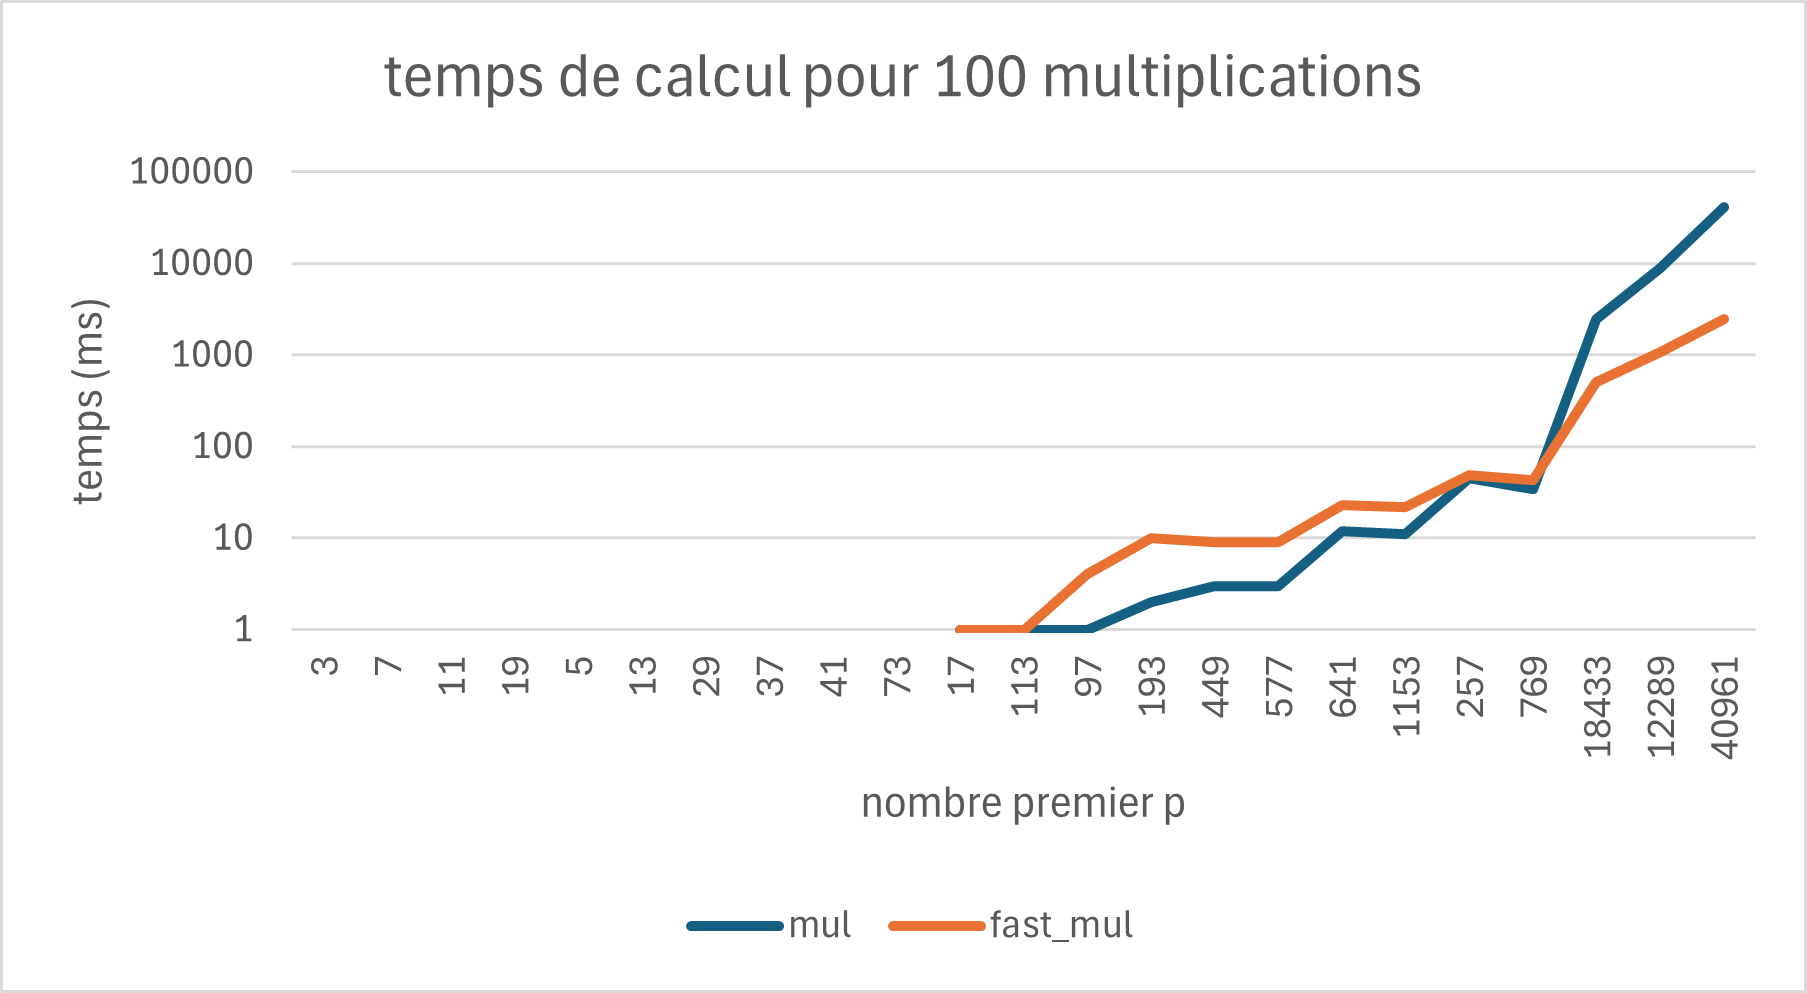
\includegraphics[width=\textwidth]{RS_mul.png}
    \end{minipage}%
    \begin{minipage}{.5\textwidth}
        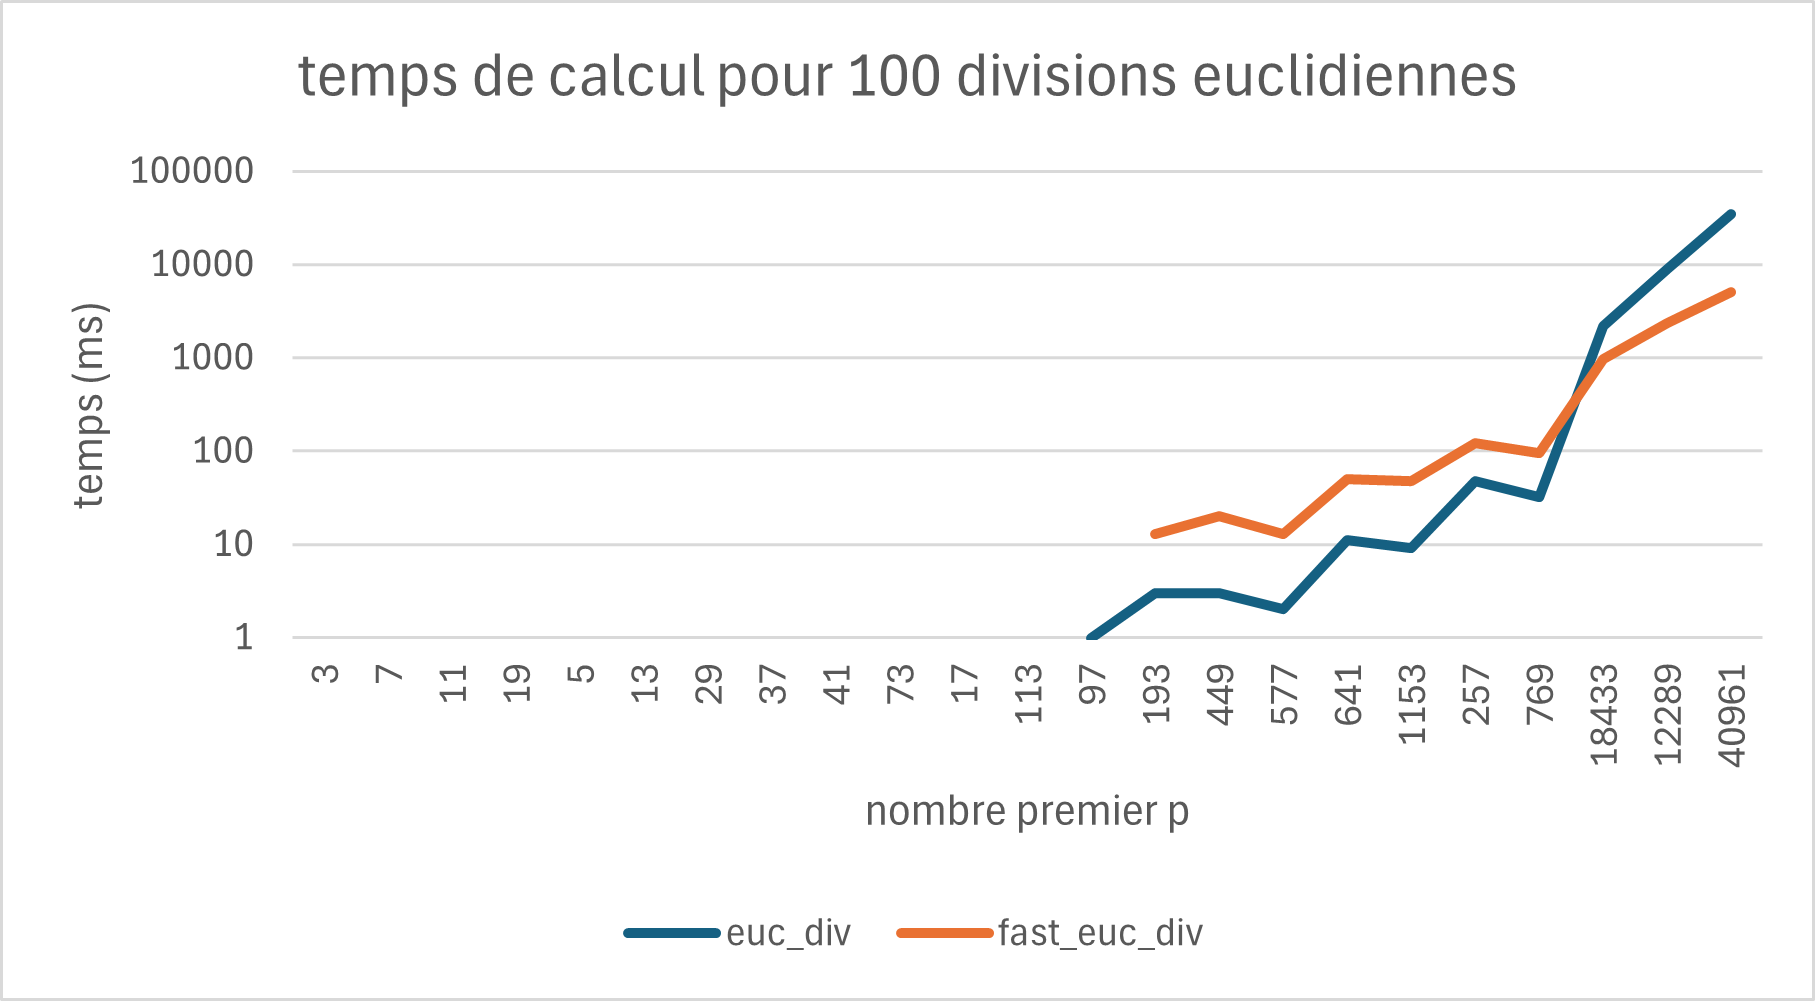
\includegraphics[width=\textwidth]{RS_div.png}
    \end{minipage}
\end{figure}

\begin{figure}
    \centering
    \begin{minipage}{.5\textwidth}
        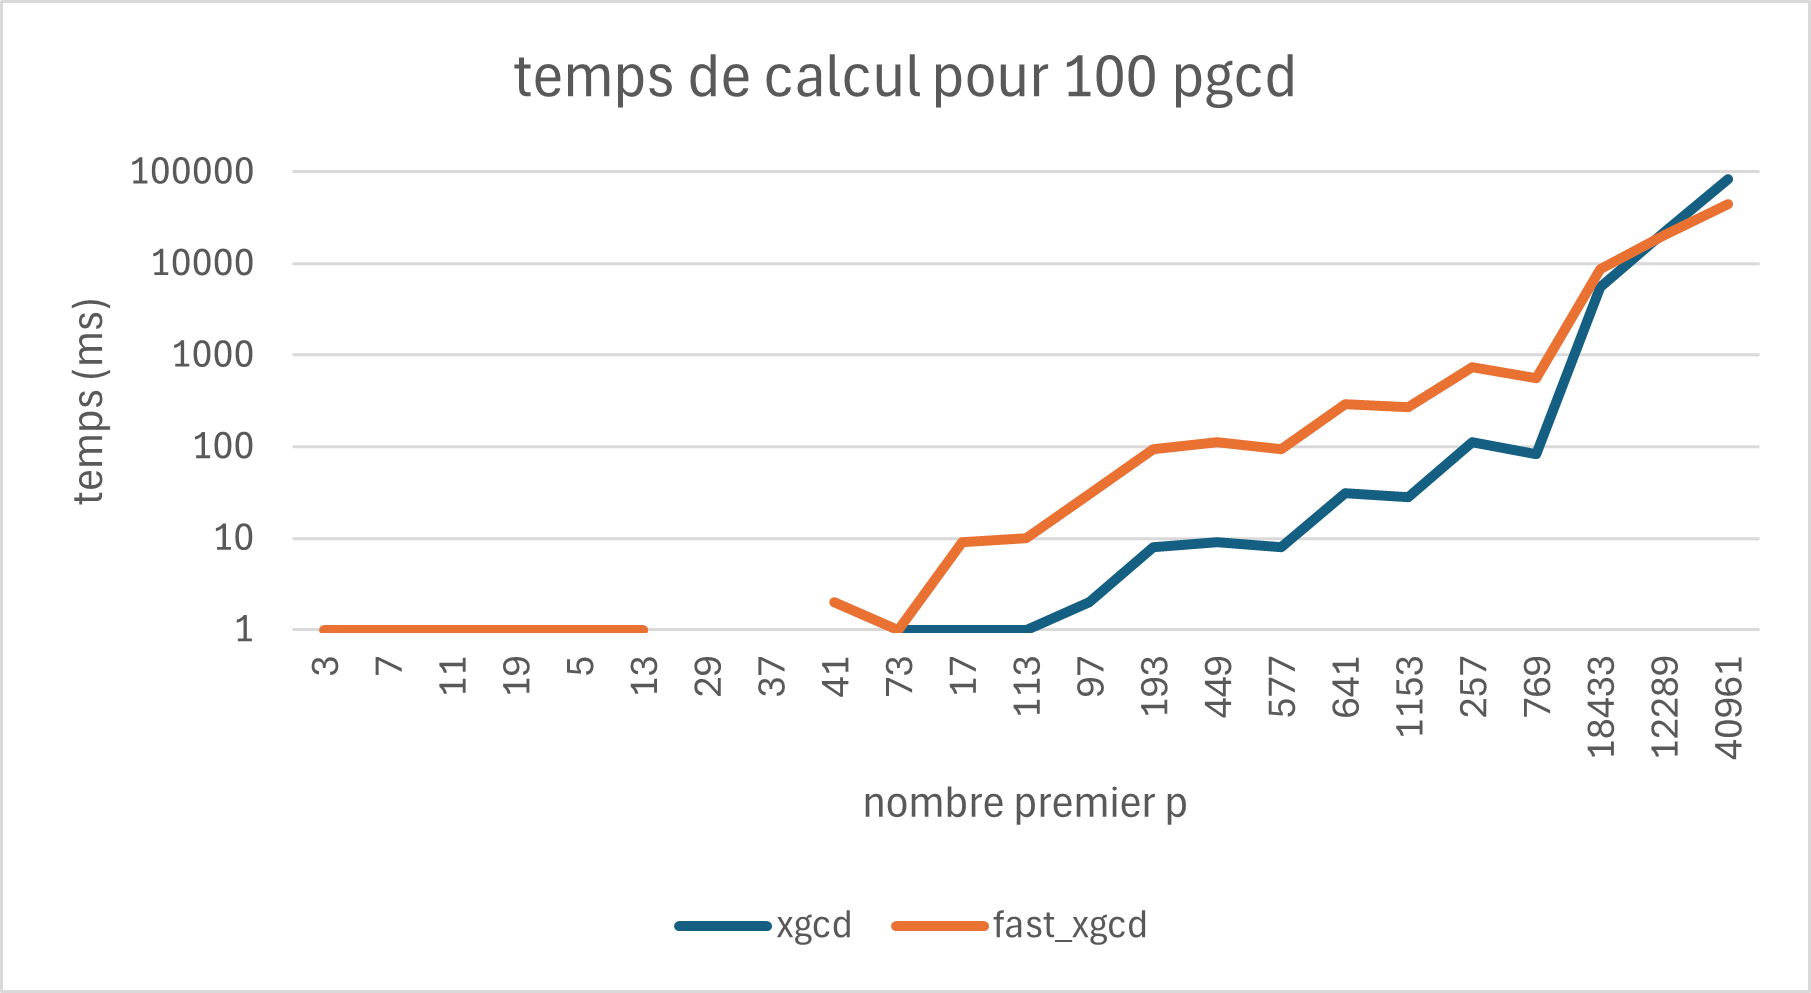
\includegraphics[width=\textwidth]{RS_gcd.png}
    \end{minipage}
\end{figure}

\begin{figure}
    \centering
    \begin{minipage}{.5\textwidth}
        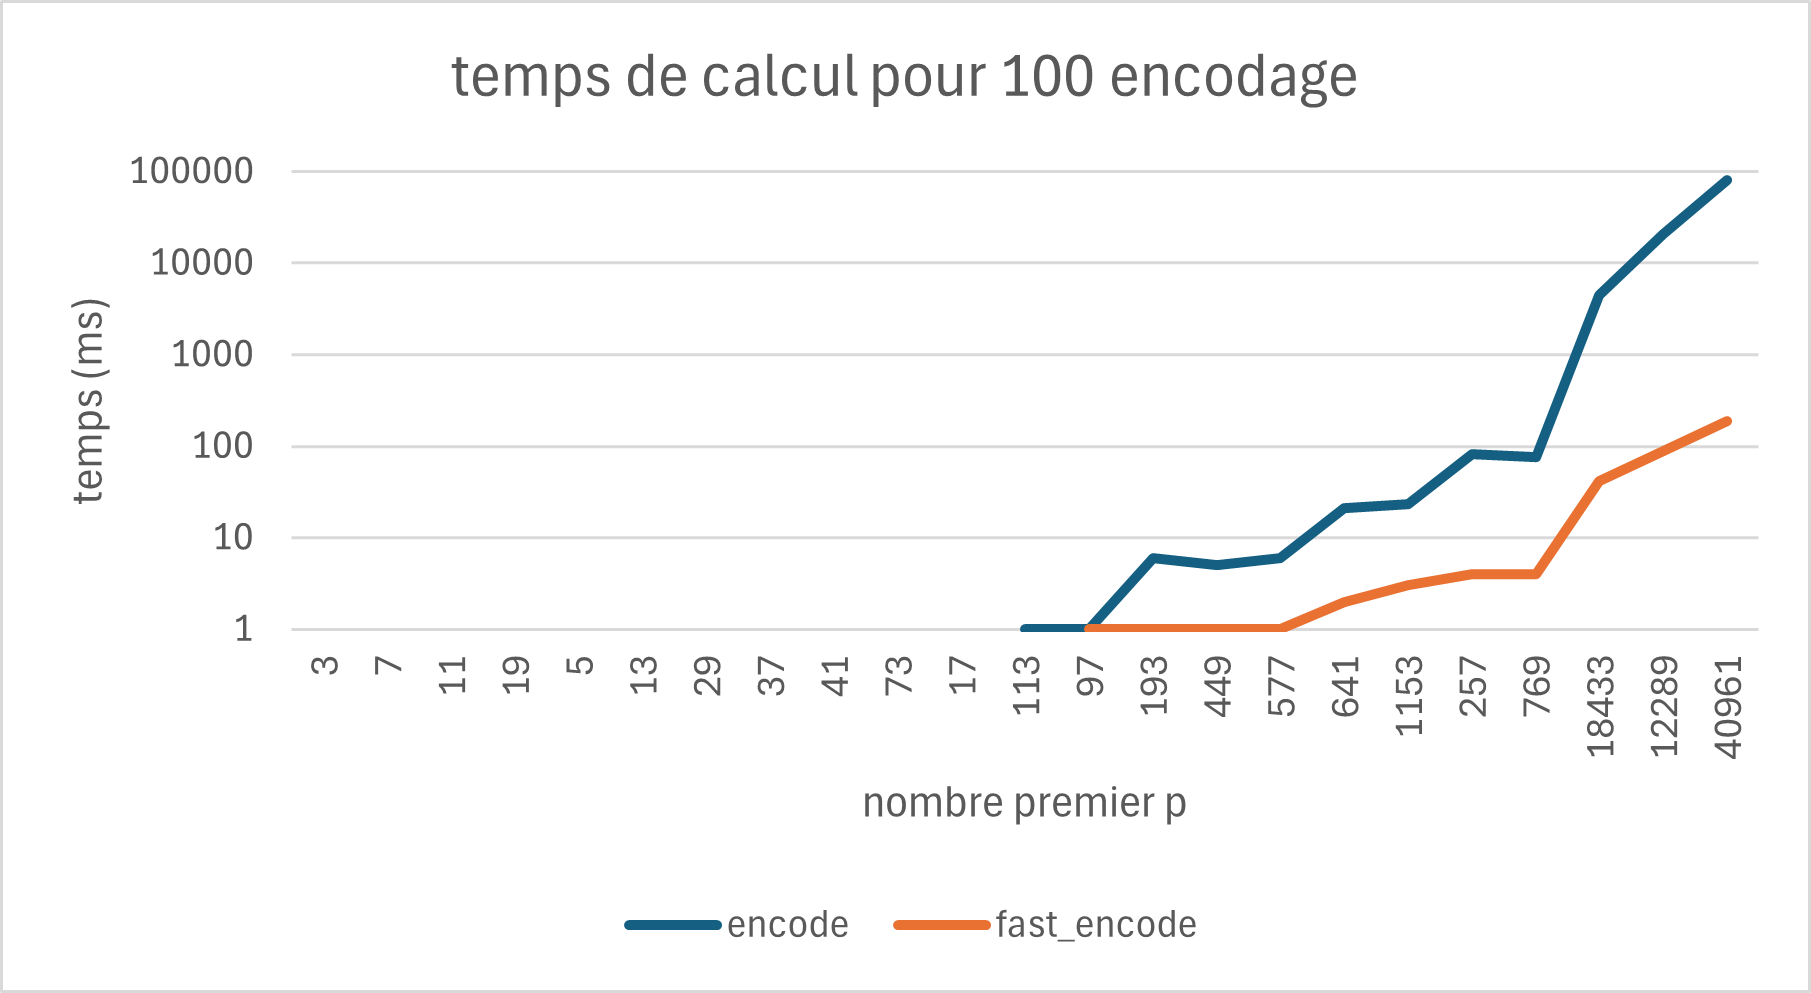
\includegraphics[width=\textwidth]{RS_enc.png}
    \end{minipage}%
    \begin{minipage}{.5\textwidth} 
        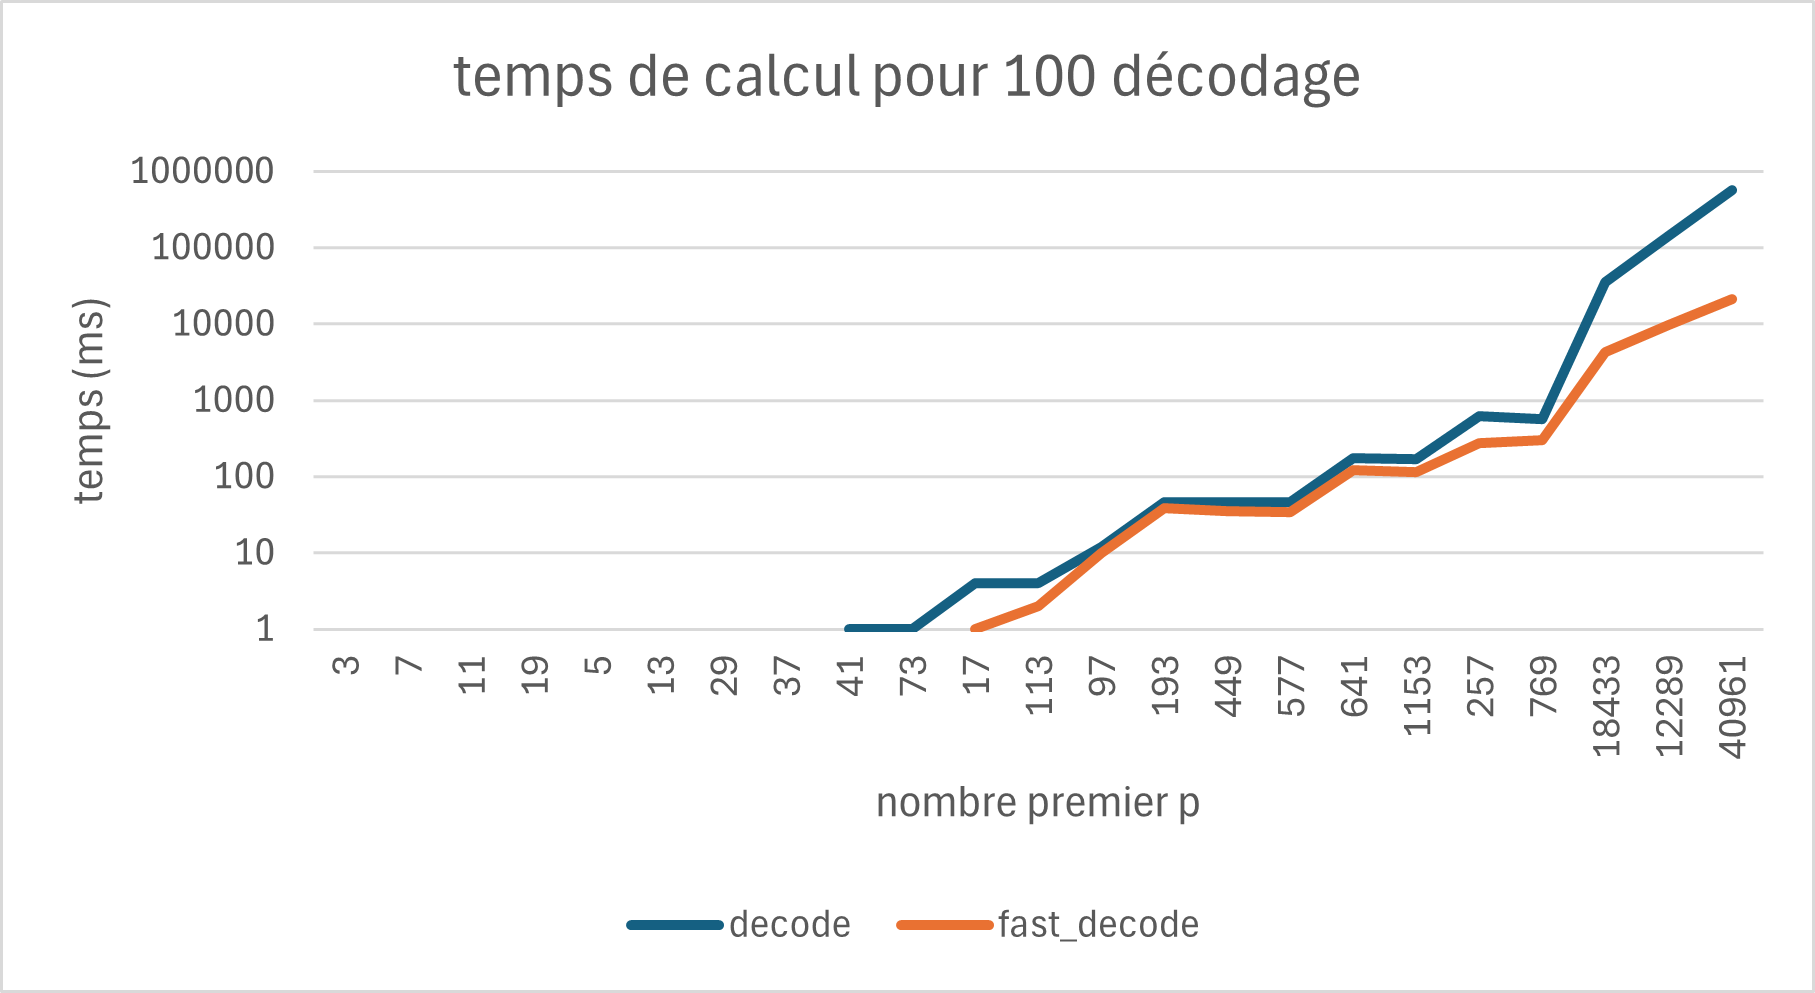
\includegraphics[width=\textwidth]{RS_dec.png}
    \end{minipage}
\end{figure}

\newpage

A cause de l'échelle logarithmique, les temps nuls (inférieurs à $1$ms) ne sont pas affichés.

On constate que pour \verb|poly_fast_mul| que le temps d'exécution est légèrement plus élevé que pour \verb|poly_mul| pour les petites valeurs de $p$. En revanche la tendance s'inverse pour les grandes valeurs de $p$. Comme annoncé par Gao la multiplication rapide devient intéressante à partir de $k \ge 8$. Pour \verb|poly_fast_euc_div| et \verb|poly_fast_xgcd| on observe le même phénomène mais avec des valeurs de $k$ plus grandes. Cela correspond bien aux complexités annoncées. Le fait que les versions \verb|fast| soient plus lentes pour des petites valeurs de $k$ n'est pas contradictoire à cause des constantes cachées dans le $\mathcal{O}$. 

Concernant \verb|rs_fast_encode| et \verb|rs_fast_decode|, on constate une très nette amélioration.


\newpage

\newgeometry{margin=2cm}
\begin{landscape}

\appendix

\section*{Résultats}

\begin{table}[!ht]
    \centering
    \begin{tabular}{c|c|c|c|c|c|c|c|c|c|c}
        \textbf{p} & \verb|mul| & \verb|fast_mul| & \verb|euc_div| & \verb|fast_euc_div| & \verb|xgcd| & \verb|fast_xgcd| & \verb|encode| & \verb|fast_encode| & \verb|decode| & \verb|fast_decode| \\ \hline
        3 & 0 & 0 & 0 & 0 & 0 & 1 & 0 & 0 & 1 & 0 \\ 
        7 & 0 & 0 & 0 & 0 & 0 & 1 & 0 & 0 & 0 & 0 \\ 
        11 & 0 & 0 & 0 & 0 & 0 & 1 & 0 & 0 & 0 & 0 \\ 
        19 & 0 & 0 & 0 & 0 & 0 & 1 & 0 & 0 & 0 & 0 \\ 
        5 & 0 & 0 & 0 & 0 & 0 & 1 & 0 & 0 & 1 & 0 \\ 
        13 & 0 & 0 & 0 & 0 & 0 & 1 & 0 & 0 & 0 & 1 \\ 
        29 & 0 & 0 & 0 & 0 & 0 & 0 & 0 & 0 & 0 & 0 \\ 
        37 & 0 & 0 & 0 & 0 & 0 & 0 & 0 & 0 & 0 & 0 \\ 
        41 & 0 & 1 & 0 & 0 & 0 & 2 & 0 & 0 & 1 & 0 \\ 
        73 & 0 & 0 & 0 & 0 & 1 & 1 & 0 & 0 & 1 & 0 \\ 
        17 & 1 & 1 & 0 & 0 & 1 & 9 & 0 & 0 & 4 & 1 \\ 
        113 & 1 & 1 & 0 & 0 & 1 & 10 & 1 & 0 & 4 & 2 \\ 
        97 & 1 & 4 & 1 & 0 & 2 & 30 & 1 & 1 & 12 & 10 \\ 
        193 & 2 & 10 & 3 & 13 & 8 & 93 & 6 & 1 & 46 & 38 \\ 
        449 & 3 & 9 & 3 & 20 & 9 & 112 & 5 & 1 & 46 & 35 \\ 
        577 & 3 & 9 & 2 & 13 & 8 & 94 & 6 & 1 & 46 & 34 \\ 
        641 & 12 & 23 & 11 & 50 & 31 & 288 & 21 & 2 & 175 & 120 \\ 
        1153 & 11 & 22 & 9 & 48 & 28 & 267 & 23 & 3 & 170 & 113 \\ 
        257 & 45 & 49 & 47 & 121 & 111 & 732 & 81 & 4 & 611 & 273 \\ 
        769 & 34 & 43 & 32 & 95 & 83 & 555 & 76 & 4 & 560 & 296 \\ 
        18433 & 2478 & 508 & 2172 & 959 & 5565 & 8664 & 4455 & 41 & 35541 & 4256 \\ 
        12289 & 8814 & 1064 & 8823 & 2328 & 21869 & 20355 & 20861 & 89 & 142067 & 9759 \\ 
        40961 & 41136 & 2456 & 34960 & 5029 & 84122 & 44924 & 80022 & 189 & 565225 & 21183 \\ 
    \end{tabular}
    \caption{Résultats des tests de performances en millisecondes}
    \label{res}
\end{table}

\end{landscape}
\restoregeometry

\bibliographystyle{unsrt}
\bibliography{biblio}

\end{document}
